\documentclass{ueacmpstyle}
\usepackage[square]{natbib}
\usepackage{enumerate}

\begin{document}
\title{CMPMP2Y --- Dissertation Proposal \\ Procedural Generation of Dungeons}
\author{Olivier Legat \\ Supervisor: Prof. Andy Day}
\maketitle

\begin{abstract}
The use of procedurally content generation (PCG) is not un-common amongst games. PCG algorithms notably present the advantage of providing potentially infinite content for the players. However, implementing a good PCG algorithm that generates convincing results is not a trivial task. This proposal discusses how to undertake a project that implements a PCG algorithm that generates a 3D interact-able environment for a dungeon-like game.
\end{abstract}

\pagebreak

\tableofcontents

\pagebreak

\section{Introduction}
Level design is a crucial factor in video games that has been around for as long as games have. It consists of manually designing an environment by specifically defining every bit of detail and importing them directly into the game. Such details include, but are not limited to: Terrain shape, goals or mission objectives, location of enemies and collectible objects.

However, level designing is not the only method to create the virtual environment of a video game. Another method is to procedurally generate a virtual environment. The concept behind this method is to write an algorithm that will design a level based on randomly generated numbers. Note that the procedural method can also be referred to as level designing, but to avoid ambiguity between the two approaches they will be referred to as {\em level designing} and {\em level generation} respectively.

Level generation is not a particularly new concept. It has been around for a significant amount of time and is present in a considerate number of existing games. Some games such as Borderlands and Left 4 Dead will have pseudo-random levels, where the overall layout of the game's level is designed by hand with certain random elements to it \citep{DBLP:journals/tciaig/TogeliusYSB11}. Other games such as Diablo will completely discard level designing and generate all the levels, enemies and props at random \citep{Nitsche-CaseStudy}.

Naturally, this programming-oriented method differs greatly from the traditional level design that is more directed towards an artistic path.

\subsection{Purpose and motivation}
The programmatic approach presents various advantages over level designing. Two major advantages are:
\begin{itemize}
\item {\bf Time:} As mentioned previously, level designing is a very time-consuming process. However, computers are much faster than humans. Once a good level generator is complete it can potentially generate an infinite amount of levels in a very short time-span. 

\item {\bf Amount of content:} As the direct result from the time constraint, level generation offers far more content. Video games with a fixed level design offer far less re-playability than those with procedural level generation because the game will get boring and predictable after a while. Level generation can allow a completely different feel to the game every-time it's played and can offer seemingly endless content \citep{DBLP:conf/aiide/ComptonM06}.
\end{itemize}

Notably, other minor advantages can emerge from this programming approach. For instance, the total memory consumption of the game when distributed could be less, because content is generated on the fly when needed and doesn't have to be packed into the distribution medium \citep{DBLP:journals/tciaig/TogeliusYSB11}.

\subsection{Statement of problem}
Although manually designing a level is far more flexible and easy than generating one, it often requires a lot time and skilled people. Level generation is often considered more challenging than level designing. Level generation is more than just generating terrain or buildings. A generator often needs to take other factors into account. Some examples include mission objectives, objects the players can interact with, spawning enemies, and so on. The general term for random content creation in a game can be referred to as Procedural Content Generation (PCG) \citep{DBLP:journals/tciaig/AshlockLM11}.

These factors are often very specific to the type of game. Because of this, most existing generic algorithms for level generation do not take these factors into account. Additionally, another issue is that most algorithms are based around 2 dimensions for simplicity and not many 3D algorithms have been implemented.

\subsection{Aim and objectives}
When reading different articles I noticed that the different methods were all focused on a specific type of environment or on a specific game. In my dissertation, I will primarily focus on generating underground dungeons but I will insure to keep the code as generic as possible so that it can be used in a number of different games. I will also be attempting to implement a 3D-based algorithm since these appear to lack much in the industry.

Overall, the summarised objectives are as follows:
\begin{itemize}
\item Develop an algorithm for random dungeon generation in 3-D.
\item Take game features such as interact-able objects, enemies and so forth into consideration.
\item Keeping the algorithm unspecific to a certain game. In other words, generalising it as much as possible.
\end{itemize}

\section{Short history}
Procedural content generation increases the amount of content or the value of a game. For this reason, it is not uncommon for games to include some form of PCG.

\begin{figure}[h!]
  \centering
    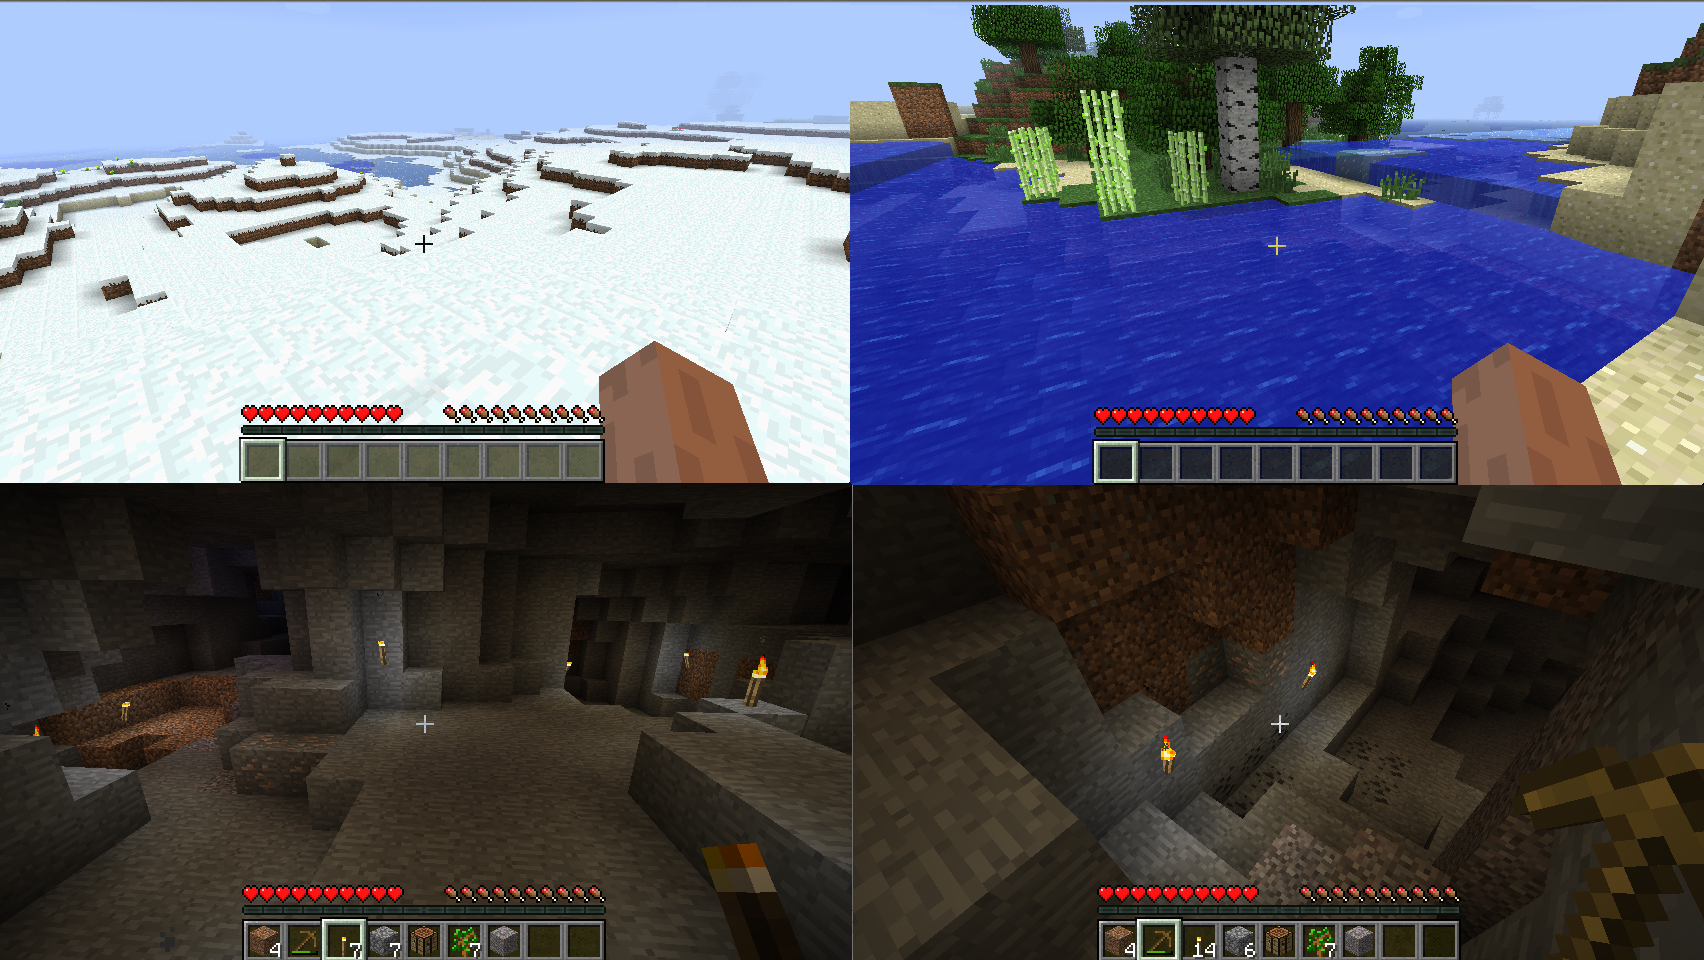
\includegraphics[width=1.0\textwidth]{images/minecraft.png}
\caption{Procedural level design in Minecraft. Everything in the environment presented is generated at random, apart from the torches. Those were placed to illuminate the underground caves.}
\end{figure}

One notable example is Minecraft, a game originally designed by the Swedish developer Markus Persson (a.k.a ``Notch") who later founded the game studio Mojang \footnote{http://www.minecraft.net/game/credits (Date accessed: 28th Feburary)}. In Minecraft, the player is placed in a world composed of different types of blocks. The blocks are placed at random using Perlin noise \footnote{http://pcg.wikidot.com/pcg-games:minecraft (Date accessed: 28th Feburary)}. The wide range of block types allows the player to experience different biomes.  The world is pseudo-infinite; meaning that as the player moves into unexplored areas the game will automatically generate more content to fill that area.

A similar game to Minecraft that also uses PCG is Terraria. Like Minecraft, it also revolves around randomly positioned blocks, with the main difference being that it's a 2D game. Terraria is a lot more focused on generating content other than terrain. In Terraria players can encounter numerous different types of enemies and can find treasure in vases and chests that are scattered across the world.
\begin{figure}[h!]
  \centering
    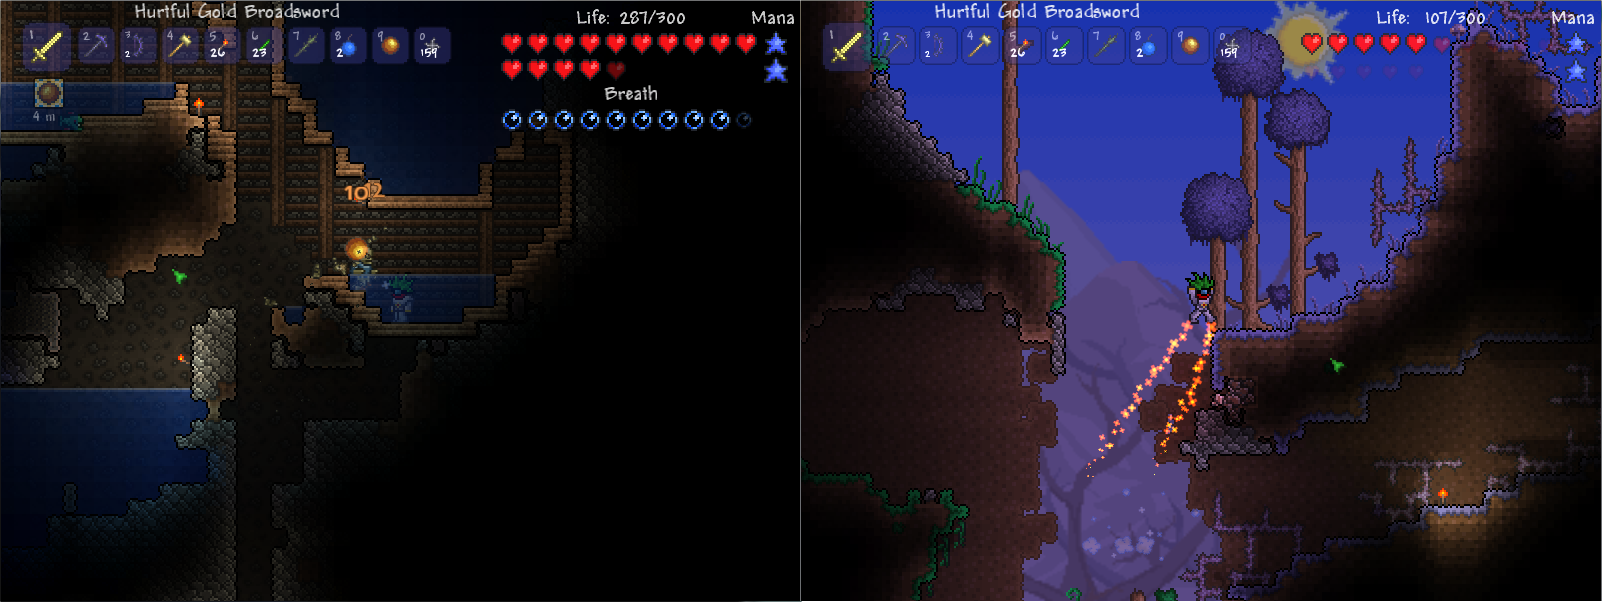
\includegraphics[width=0.7\textwidth]{images/terraria.png}
\caption{Terraria is a 2D game inspired by Minecraft which also utilises PCG.}
\end{figure}

\section{Literature review}
The literature review will examine how existing algorithms work and extract key elements from them. There are various articles that explore a numerous amount of different methods to generate levels. Here are some examples of such methods:






\section{Evaluation}
Many interesting techniques have been discussed in the literature review on how to procedurally generate content for a video game. Sadly, not all of these techniques can be applied in the dissertation together. For instance, the rhythm-based approach is too aimed towards platform games. The notion of rhythm in different game genres, such as shooting games, is perhaps less important. Therefore the rhythm-based technique cannot be used to conceive generic algorithm in the scope of this dissertation. 

\subsection{Focus}
Although the one of the aims of my dissertation is to develop a generic algorithm it will focus specifically on {\em dungeon-like} environments. The reason for this specialisation is that algorithms which target a specific type a problem often provide more satisfying result than those which generalise over different types of problems. 

A genetic algorithm approach can allow a descent amount of generalisation through the use of an abstract fitness function. Therefore, a generic algorithm would be an interesting approach because it would allow users to be even more specific as to how the dungeon should look like. Rhythm-based PCG won't be directly supported since those algorithms are mainly aimed at 2D plat-forming games. However, with the use of an abstract fitness function it could potentially be possible for the user to specify how to generate a rhythm-based environment. Unfortunately genetic algorithms are notoriously slow \citep{DBLP:conf/cig/TogeliusPBWHY10}, thus generating content in real-time isn't a key objective.

Another key focus point of this dissertation is to generate a 3D dungeon. Naturally, the algorithm will have to consider some sort of procedural modelling in order to pass vertices to graphics device. This can be done using some techniques discussed in the literature review. Rendering the environment efficiently is also a crucial factor. Basic concepts such as view-frustum culling, vertex and index buffer objects should be used. The algorithm should avoid generating high-poly meshes to save render-time and memory. Additionally the environment should be appropriately textured and the texturing process should remain generic.

The generator will be based around the concept that a dungeon consists of {\em rooms} and {\em corridors}, somewhat like an indirect negative representation of a maze-like level \citep{DBLP:journals/cim/AshlockLM11}. Rooms can be constructed using Greuter et al.'s method of building a floor-plan \citep{DBLP:conf/graphite/GreuterPSL03} or using an occupancy-regulated algorithm \citep{DBLP:conf/cig/MawhorterM10}. These two classes can be sub-classed to specify different types of rooms or corridors. Krecklau et al. have presented an interesting way to interconnect structures using inverse kinematics, this could be used the generate the corridor that connect rooms together \citep{DBLP:journals/cgf/KrecklauK11}. Additional content, such as doors, traps and so forth will be generated in post-processing because they are specific to a certain game.

\subsection{Work-plan}
The project will be developed using agile programming methods. This means that the aim is to get minimal working software done as soon as possible. Features will then be added or enhanced based upon existing code. These are the steps that will be taken in the development process:

\begin{enumerate}
\item {\bf Initialisation: } This consists of getting a very primitive environment generated at random from scratch. If a generic algorithm is going to be used then some data must already exist in order to evolve it. The initialisation algorithm will simply place random rooms at random positions in a 3D space and randomly link them together. The precise randomisation methods will remain abstract in order to keep the initialisation generic.
\item {\bf Evolving: } Once the initial dungeon is complete it will be time to enhance its features based on a fitness function. Again, the evolution process will remain as abstract as necessary to keep the whole project generic.
\item {\bf Post-processing: } This phase consists of adding anything extra thing which cannot be generalised. This phase is the least important and will mainly be used for the purpose of demonstration.
\end{enumerate}

\subsection{Risk analysis}
\begin{itemize}
\item {\bf Hard-drive failure: } The impact of a hard-drive failure or lose is very severe and often un-resolvable if a back-up doesn't exist. For this reason, I will keep various back-up copies of my work. I will frequently copy content from my laptop's hard disk onto my external back-up drive. Additionally, I will store all work on a Sub-version (SVN) server to back-up my work.
\item {\bf Software developement delay: } Development delay is very common. In most cases when it occurs, some software features need to be cut down. To avoid having this done I will always make sure to leave empty days in my schedule to allow myself to catch up and remain on time. Naturally, if this doesn't work then some features will inevitably have to be removed.
\item {\bf Overly complex task: } It is possible that as time proceeds I will realise that the problem is more complicated than I anticipated and won't be complete on time. This will generally occur towards the end of the project. Since the development process will be done using an iterative approach, working software will be available early on. If I cannot expand the software to reach it's initial requirements it will likely need to be simplified, by adding constraints or making assumptions, and the issues would be discussed to explain why the problem had to be narrowed down. However, if this problem is encountered early on then an alternative method should quickly be revised.
\item {\bf Minor Illness: } Small illnesses, such as a cold, will only last a short period and will not have a major impact. Leaving some empty days in the schedule will generally compensate for this.
\end{itemize}

\section{Conclusion}
Many PCG techniques have been discussed and genetic algorithms seem to be very popular amongst them. Sadly, they do not seem do be frequently used in real-time applications due to their inefficiency. We have observed that complicated PCG algorithms can be divided into set of simpler steps. The various techniques used will be used to implement a hybrid algorithm. Random rooms is will be procedurally modelled then inter-connected using IK \citep{DBLP:journals/cgf/KrecklauK11}. The overall dungeon will then be enhanced by a genetic algorithm.

\pagebreak
\appendix
\section{Appendix}
\begin{figure}[h!]
  \centering
    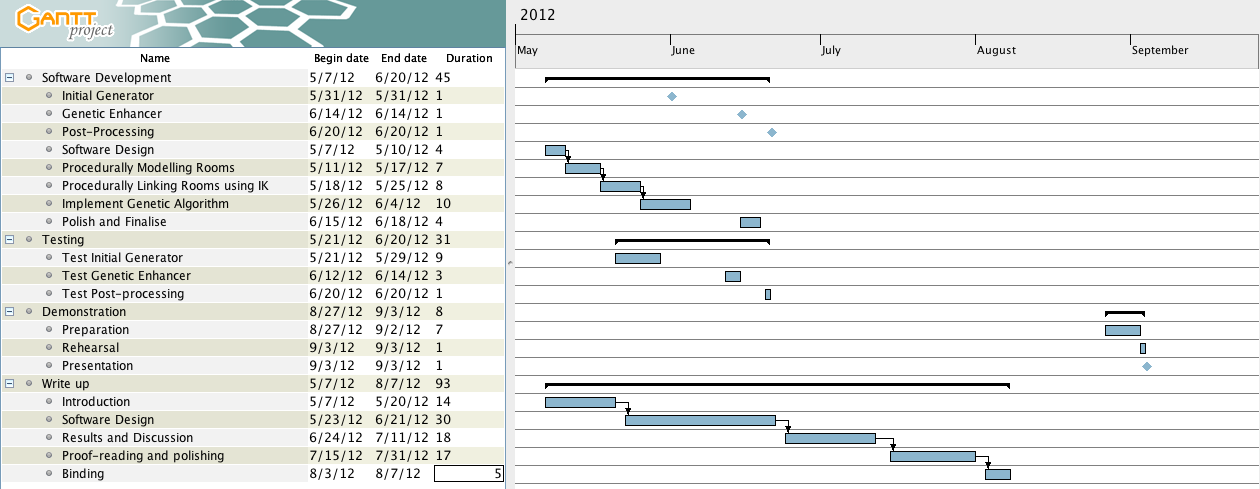
\includegraphics[angle=90, width=0.5\textwidth]{images/workplan.png}
  \caption{Work-plan for the dissertation.}
\end{figure}

\pagebreak
\bibliographystyle{apalike}
\bibliography{MyBib}


\end{document}
